\documentclass[UTF8,a4paper,11pt,fontset=none]{ctexart}

\usepackage{geometry}
\usepackage{hyperref}
\usepackage{xcolor}
\usepackage{enumitem}
\usepackage{listings}
\usepackage{graphicx}
\graphicspath{{figures/}{../figures/}}

\setCJKmainfont{Noto Serif CJK SC}[
  BoldFont = Noto Serif CJK SC Bold,
  ItalicFont = Noto Serif CJK SC
]
\setCJKsansfont{Noto Sans CJK SC}[
  BoldFont = Noto Sans CJK SC Bold
]
\setCJKmonofont{Noto Sans Mono CJK SC}

\geometry{left=2.45cm,right=2.45cm,top=2.35cm,bottom=2.35cm}
\hypersetup{
  colorlinks=true,
  linkcolor=blue!55!black,
  urlcolor=blue!55!black
}

\setlength{\parindent}{0pt}
\setlength{\parskip}{0.55em}
\setlist[itemize]{leftmargin=2em,itemsep=0.18em,topsep=0.2em}
\setlist[enumerate]{leftmargin=2em,itemsep=0.18em,topsep=0.2em}
\raggedbottom
\sloppy

\lstset{
  basicstyle=\ttfamily\small,
  breaklines=true,
  columns=fullflexible,
  frame=single,
  rulecolor=\color{black!25},
  backgroundcolor=\color{black!3}
}

\newcommand{\skill}[1]{\texttt{#1}}
\newcommand{\file}[1]{\texttt{#1}}
\newcommand{\cmd}[1]{\texttt{#1}}
\newcommand{\keypoint}[1]{\textbf{#1}}

\title{\textbf{Codex 使用指南}\\{\large Goal、Subagent 与本地 Skills 工作流}}
\author{本地 Codex 工作流手册}
\date{2026-06-30}

\begin{document}
\maketitle
\thispagestyle{empty}
\newpage
\tableofcontents
\newpage

\section{报告边界与阅读顺序}

Codex 不是一个只回答问题的聊天窗口，而是一个和你共享工作区的工程协作者。它可以读仓库、改文件、运行命令、查看日志、维护任务文档，并在需要越过沙箱或访问外部资源时请求批准。

这份报告可以作为 GitHub 使用指南仓库的正文，也可以作为本地 PDF 手册。它按“先通用方法，后场景 skills，最后本机实现映射”的顺序写。前半部分先解释 Goal、subagent、\file{AGENTS.md}、任务请求和验证闭环，这些内容适用于大多数 Codex 项目；后半部分再说明工程、学术场景，最后一节才说明本机 Goal 入口的对应实现。

\subsection{这份指南适合谁}

这份指南同时服务两类读者：

\begin{itemize}
  \item \keypoint{初学者}：先理解 Codex 能做什么、如何描述任务、如何判断完成、如何避免把权限和验证交给模型自由发挥。
  \item \keypoint{进阶用户}：重点关注 Goal、subagent、\file{AGENTS.md}、skills、团队化审查和可复现交付，目标是把 Codex 用成一个能沉淀流程的工程协作者。
\end{itemize}

初学者不需要先掌握所有本机 skills。先学会写清目标、范围、约束和验证，就已经能显著提高 Codex 输出质量。进阶用户则应该进一步关心上下文隔离、subagent 输出合同、Goal closeout、项目规则复用和证据边界。

阅读顺序建议如下：

\begin{enumerate}
  \item \keypoint{初学者路线}：第 1、2、3、6、7、10 节。先掌握 Codex 工作面、Goal 写法、项目规则、日常请求和模式选择。
  \item \keypoint{进阶路线}：第 3、4、5、6、8、9、12 节。重点看 Goal、subagent、组合模式、工程/学术 skills 和本机实现映射。
  \item \keypoint{维护者路线}：第 11、12 节，再回到 \file{README.md}、\file{CONTEXT.md} 和 \file{docs/adr/}，保证仓库适合公开发布和后续更新。
\end{enumerate}

本文保留英文固定名，例如：

\begin{itemize}
  \item \file{AGENTS.md}、\file{SKILL.md}；
  \item \skill{grill-me}、\skill{ask-research}；
  \item \skill{subagent-driven-development}、\cmd{make pdf}。
\end{itemize}

中文解释用于说明它们在本机工作流里的作用。

\subsection{零基础 10 分钟上手}

如果你第一次使用 Codex，不需要先理解所有 Goal、subagent 和 skills。先按下面这个最小闭环操作：

\begin{enumerate}
  \item \keypoint{打开项目}：在 Codex app 中选择一个明确的项目文件夹，不要在一个无关的大目录里开始。
  \item \keypoint{用四段式提问}：写清目标、范围、约束、验证。哪怕只写四行，也比一句“帮我优化”可靠。
  \item \keypoint{让 Codex 先读上下文}：要求它读取 \file{AGENTS.md}、\file{README.md}、相关源码或 \file{SKILL.md}，再开始改。
  \item \keypoint{只批准你看得懂的命令}：下载依赖、联网、写工作区外目录、删除文件、长期运行服务都要谨慎。
  \item \keypoint{看证据而不是看承诺}：结束时检查 diff、测试、构建、日志、PDF、截图或其它可观察产物。
\end{enumerate}

\begin{figure}[htbp]
  \centering
  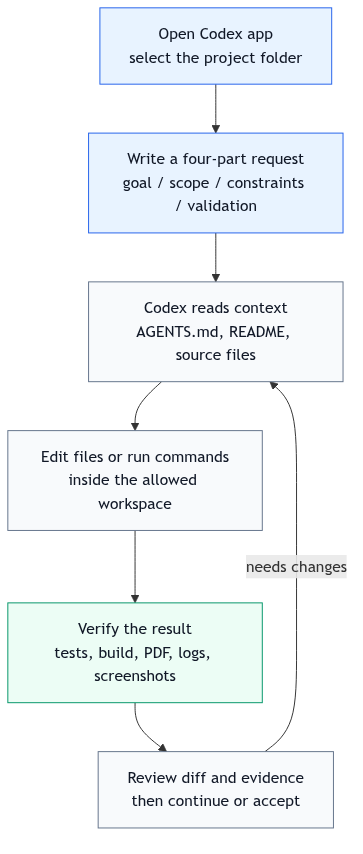
\includegraphics[height=0.46\textheight]{beginner-quickstart.png}
  \caption{零基础用户的最小 Codex 使用闭环}
\end{figure}

最小请求模板如下：

\begin{lstlisting}
在这个项目里做一件事：<目标>。
范围：只改 <路径/模块>，不要动 <排除范围>。
约束：<语言、格式、API、字段、权限、风格等硬约束>。
验证：完成后请运行 <命令/检查>，并告诉我改了哪些文件、验证结果和剩余风险。
\end{lstlisting}

如果你不知道验证命令，也可以写“请先读项目说明，找出最窄的验证方式，再执行”。这比完全不提验证更好。

\subsection{作为 GitHub 仓库的发布边界}

如果把这份材料发布到 GitHub，仓库应当让读者先在 \file{README.md} 里看懂三件事：这是什么、适合谁、怎么生成 PDF。正文 PDF 负责系统讲解；\file{CONTEXT.md} 负责术语；\file{docs/adr/} 负责记录为什么采用“通用方法优先、场景 skills 其次、最后实现映射”的结构。

构建产物建议通过 GitHub Releases 或 CI artifact 发布，而不是把 \file{build/} 目录提交进仓库。这样读者可以复现 PDF，仓库也不会被二进制文件污染。

\section{Codex 的工作面}

选择 Codex 入口时，不要只看“能不能让模型写代码”，而要看任务需要什么样的上下文、交互、权限和可追踪性。

\begin{itemize}
  \item \keypoint{Codex app}：适合桌面端规划、审查、并行 threads、diff、终端、in-app browser、Computer Use、worktree、automations 和多项目切换。官方页面把它描述成面向 Codex threads 的桌面端 focused experience，并强调 worktrees、automations 和 Git 功能。
  \item \keypoint{Local / Worktree}：适合在 Desktop 里选择当前项目或隔离工作区，让 Codex 在可审查的范围内读写、验证和提交。
  \item \keypoint{Integrated terminal}：适合在 Desktop 线程里运行测试、构建、链接检查和发布验证，并把输出作为同一个任务的证据。
  \item \keypoint{IDE Extension}：适合编辑器内联上下文、代码定位和编辑器同步。
  \item \keypoint{Codex web/cloud}：适合 hosted 或 offloaded 工作、远程环境、PR review 或云端任务。
\end{itemize}

本指南主要面向 Codex app + 本地仓库的组合：你在 app 里选择项目文件夹，Codex 在本机工作区内读写文件，必要时通过终端运行验证命令。

\subsection{Codex app 的实际工作循环}

Codex app 的强项不是“聊天”，而是把工程循环放在同一个界面里：

\begin{itemize}
  \item 选择项目文件夹；
  \item 在 thread 里解释任务、约束、边界；
  \item 让 Codex 读文件、改文件、运行命令；
  \item 在 diff/review 面板里看改动；
  \item 对失败测试、排版问题、浏览器结果继续反馈；
  \item 必要时用 worktree、subagent、automation 或 goal mode 扩大执行能力。
\end{itemize}

因此，一个好的 Codex 请求不只是“帮我做一下”，而是把“目标、范围、约束、验证、交付物”写清楚。任务越长，越要写成可执行合同；任务越短，越要防止过度流程化。

\subsection{三类上下文}

Codex 的表现取决于它拿到的上下文质量。常见上下文可以分成三类：

\begin{itemize}
  \item \keypoint{用户上下文}：当前消息、口头约束、语言偏好、优先级排序。
  \item \keypoint{项目上下文}：\file{AGENTS.md}、\file{README.md}、\file{CONTEXT.md}、ADR、测试命令、代码结构。
  \item \keypoint{执行上下文}：当前工作目录、沙箱权限、Git 状态、命令输出、构建产物、截图、日志。
\end{itemize}

很多失败不是模型不会写代码，而是上下文边界没建立好。例如没有说明不能改公开 API、没有告诉它哪个目录是目标路径、没有要求重新编译 PDF，最后就会出现“代码像完成了，但交付物没验证”的问题。

\section{Goal 模式先讲清楚}

Goal 模式适合长任务、跨阶段任务、需要可追踪 artifact 的任务。它比普通会话更重，因为它维护目标、准备检查、上下文、团队、调度、验证和 closeout。一个 Goal 不是标题，而是一份执行合同。

普通会话适合：

\begin{itemize}
  \item 单个问题；
  \item 小范围文件修改；
  \item 一两个命令即可验证的任务；
  \item 不需要跨阶段追踪的讨论。
\end{itemize}

Goal 模式适合：

\begin{itemize}
  \item 多阶段实现或长期实验；
  \item 需要 subagent 或专家团队；
  \item 需要记录 work queue、artifact、验证证据；
  \item 可能中断、恢复、交接的任务；
  \item 高风险任务，例如论文证据边界、跨模块重构、部署、分支收尾。
\end{itemize}

\subsection{一个 Goal 要回答的核心问题}

写 Goal 时，先回答这些问题：

\begin{enumerate}
  \item \keypoint{到底要完成什么？} 目标必须是可观察结果，不是愿望。
  \item \keypoint{在哪些地方工作？} 写清仓库、目录、模块、文件、分支或实验路径。
  \item \keypoint{什么算成功？} 成功标准要能被用户、测试、构建、报告或审查确认。
  \item \keypoint{什么算验收？} 验收标准是结束前必须看到的证据。
  \item \keypoint{不能做什么？} 包括 API、字段名、路径、数据、格式、语言、权限和 destructive 操作。
  \item \keypoint{怎么验证？} 写具体命令、检查、截图、日志、PDF 抽取、指标或人工确认。
  \item \keypoint{产出什么？} 例如代码、PR、PDF、表格、实验日志、manifest、分析报告。
  \item \keypoint{什么时候必须停？} 缺数据、权限失败、结果冲突、风险越界时不要硬做。
\end{enumerate}

如果这些问题回答不出来，不要急着创建 goal。先用普通会话、\skill{grill-me}、\skill{grill-with-docs} 或 plan-only 阶段把边界压实。

\subsection{Goal objective 的字段}

一个完整 Goal objective 建议包含这些字段：

\begin{itemize}
  \item \keypoint{Objective}：一句话说明最终目标。
  \item \keypoint{Context}：重要仓库、artifact、branch、实验、论文或环境背景。
  \item \keypoint{Scope}：包括哪些路径、模块、文件或任务。
  \item \keypoint{Out of Scope}：明确排除什么，避免隐式扩张。
  \item \keypoint{Success Criteria}：完成后必须为真的状态。
  \item \keypoint{Acceptance Criteria}：验收门槛，最好能落到测试、构建、截图或报告。
  \item \keypoint{Validation}：命令、artifact、指标、审查或人工检查。
  \item \keypoint{Constraints}：硬约束，例如不改 API、不新增 JSON 字段、不移动 allowlist、中文优先。
  \item \keypoint{Deliverable}：最终回答或产物要交付什么。
  \item \keypoint{Artifacts}：运行时要保留哪些日志、manifest、PDF、表格或决策记录。
  \item \keypoint{Stop Conditions}：遇到什么情况停止并报告 blocked。
  \item \keypoint{Project Instructions}：repo-bound 工作要说明项目规则和 instruction chain 如何解析和传递。
\end{itemize}

紧凑 objective 应该控制长度，优先保留 success criteria、acceptance criteria、validation、hard constraints 和 stop conditions。如果目标太长，应该缩小范围或改成 handoff，而不是把关键验收信息删掉。

\subsection{可复制的 Goal 模板}

下面是一个通用模板，可以直接改写：

\begin{lstlisting}
Objective:
<one concrete outcome sentence>

Context:
<repo, branch, artifact, experiment, paper, environment, or user context>

Scope:
- Include: <paths/modules/tasks>
- Exclude: <explicitly out of scope>

Success Criteria:
- <state that must be true>
- <user-visible or artifact-visible result>

Acceptance Criteria:
- <observable completion gate>
- <tests/builds/reviews that must pass>

Validation:
- <commands to run>
- <manual checks or artifact checks>

Constraints:
- <must preserve>
- <must avoid>
- <language/style/security/permission boundaries>

Deliverable:
- <what final response or artifact must contain>

Artifacts:
- <logs/manifests/PDFs/screenshots/reports to keep>

Stop Conditions:
- <when to stop and report blocked>
- <when to ask the user before continuing>
\end{lstlisting}

\subsection{一个针对本文的 Goal 示例}

下面这个 objective 展示如何把“重写 PDF”写成可执行目标：

\begin{lstlisting}
Objective:
Rewrite the Codex usage guide into a roughly 20-page Chinese PDF that
puts Goal and subagent usage first, keeps at least 10 pages of general
guidance before scenario-specific skills, and ends with local skills guidance.

Context:
Repo: /home/hujie/paper/tools/codex-usage-guide.
The previous PDF compiled but needs stronger structure and more generic content.

Scope:
Edit src/main.tex, CONTEXT.md, docs/adr if needed.
Do not edit unrelated repositories.

Success Criteria:
- Goal and subagent chapters appear before scenario-specific skills.
- Goal objective writing is explained with required fields and examples.
- Later chapters explain engineering and academic skills.
- The final section maps this generic Goal/Subagent model to the local implementation.
- PDF is around 20 pages and renders Chinese correctly.

Acceptance Criteria:
- make pdf succeeds.
- pdffonts shows CJK fonts with uni=yes.
- pdftotext extracts Chinese from the first pages.
- Representative preview pages are visually readable.

Constraints:
- Chinese-first text.
- Preserve exact English identifiers.
- Keep implementation-specific Goal router details out of the generic sections.
- Do not commit unless Git identity is configured.

Stop Conditions:
- Required skill files cannot be read.
- LaTeX cannot compile after focused fixes.
- PDF still drops Chinese glyphs in preview or text extraction.
\end{lstlisting}

\subsection{Goal 的轻重分层}

不是所有目标都需要完整调度。可以按轻重分三层：

\begin{itemize}
  \item \keypoint{轻量目标}：清晰、低风险、只读检查、小改动或单命令验证。通常不需要 subagent，只需要明确完成证据。
  \item \keypoint{标准目标}：非平凡实现、调试、审查或规划。可以使用少量 subagent，但要避免过度并行。
  \item \keypoint{完整目标}：多分支、高风险、长时间、论文证据敏感、跨模块或需要独立审计的任务。需要完整 artifact、队列、团队边界、调度记录和收尾验证。
\end{itemize}

判断轻重的关键不是任务听起来“高级”，而是证据边界。一个小 bug 如果影响生产数据，可能需要标准目标；一个大文档修订如果范围清楚，可能只需要普通会话或轻量目标。

\section{Subagent 模式前置}

Subagent 是隔离上下文的专用执行者。它的价值是把探索、测试、日志分析、独立审查等 noisy work 移出主线程，让主线程保留需求、约束、决策和最终整合。

Subagent 不是“让多个模型随便干活”。它必须有明确边界、输出合同和整合点。主线程永远负责最终判断。

\subsection{什么时候使用 subagent}

适合使用 subagent：

\begin{itemize}
  \item 多个测试文件失败，根因可能互不相关；
  \item 多个子系统可以独立调查；
  \item 一个计划已经拆成清晰、互不重叠的任务；
  \item 每个任务都有明确输入、范围和输出格式；
  \item 需要独立审查，例如安全、性能、测试覆盖、论文证据边界。
\end{itemize}

不适合使用 subagent：

\begin{itemize}
  \item 失败之间高度相关，修一个可能影响全部；
  \item 需要先理解全局架构；
  \item 多个 subagent 会改同一批文件；
  \item 目标本身还没问清楚；
  \item 结果无法通过测试、日志或人工检查整合。
\end{itemize}

\subsection{如何明确要求 Codex 使用 subagent}

Codex 不应默认为每个任务创建 subagents。你要明确说“spawn agents”、“delegate in parallel”、“use one agent per point”或中文等价表达。

一个好的 subagent 请求包含四点：

\begin{itemize}
  \item 如何拆分工作；
  \item 每个 subagent 的边界；
  \item 是否等待所有 subagents 完成；
  \item 返回什么摘要格式。
\end{itemize}

可复制模板：

\begin{lstlisting}
请用并行 subagents 审查当前分支。
spawn one agent per point, wait for all of them, then summarize.

Agent 1: security risks，只读审查，不改文件。
Agent 2: missing tests，只读审查，不改文件。
Agent 3: maintainability，只读审查，不改文件。

每个 agent 返回：
- findings with file/line references
- risk level
- recommended fix
- whether it needs code change
\end{lstlisting}

\subsection{每个 subagent 都要有输出合同}

subagent prompt 至少要写清：

\begin{itemize}
  \item \keypoint{owner}：这个 agent 负责哪个问题；
  \item \keypoint{read/write scope}：只读还是允许写，能写哪些路径；
  \item \keypoint{dependency and wait strategy}：要等什么，什么时候可以继续；
  \item \keypoint{expected output contract}：必须返回哪些字段；
  \item \keypoint{integration checkpoint}：主线程在哪里整合结果；
  \item \keypoint{conflict-resolution path}：发现冲突时由谁裁决；
  \item \keypoint{fallback plan}：partial、blocked、stale、conflicting 或 unverifiable 时怎么办。
\end{itemize}

实现类 subagent prompt 可以这样写：

\begin{lstlisting}
Implement Task 2 only.

Scope:
- files: src/foo.py, tests/test_foo.py
- do not edit public API names
- preserve existing behavior unless the task says otherwise

Goal:
- add validation for empty input
- add focused tests

Return:
- status: DONE | DONE_WITH_CONCERNS | NEEDS_CONTEXT | BLOCKED
- files changed
- tests run
- evidence
- concerns
\end{lstlisting}

\subsection{并行 subagent 的边界}

并行不是越多越好。并行只适合独立问题域。每个并行分支必须有：

\begin{itemize}
  \item specific scope；
  \item clear goal；
  \item non-overlapping write scope；
  \item validation plan；
  \item expected output；
  \item integration checkpoint。
\end{itemize}

主线程整合时不能按“投票”决定，而要按证据整合：去重事实、保留冲突、区分 confirmed fact 和 inference，然后用 acceptance criteria 决定下一步。

\subsection{Goal 模式中的 subagent}

Goal-bound subagent 更严格。主 orchestrator 拥有 goal 生命周期、分支、worktree、merge、最终验证和 closeout。subagent 只拥有被分配的 task、write scope 和 output contract。

硬规则：

\begin{itemize}
  \item subagent 不管理 Goal 生命周期；
  \item subagent 不拥有 branch、worktree、merge 或 goal 生命周期；
  \item subagent 不应被分配编排协议或目标管理职责；
  \item repo-bound subagent 必须收到目标路径适用的 \file{AGENTS.md} chain；
  \item 写入范围不能重叠；
  \item 完成前主线程必须重新验证。
\end{itemize}

\subsection{自定义 subagent}

Codex 支持内建 agent，例如 \skill{default}、\skill{worker}、\skill{explorer}。也可以在 \file{\textasciitilde/.codex/agents/} 或项目内 \file{.codex/agents/} 放 TOML 文件定义自定义 agent。

最小 schema：

\begin{lstlisting}
name = "reviewer"
description = "PR reviewer focused on correctness and tests."
developer_instructions = """
Review like a code owner.
Prioritize correctness, regressions, security, and missing tests.
Return findings first with file and line references.
"""
\end{lstlisting}

常用可选字段包括：

\begin{itemize}
  \item \file{model}；
  \item \file{model\_reasoning\_effort}；
  \item \file{sandbox\_mode}；
  \item \file{mcp\_servers}；
  \item \file{skills.config}。
\end{itemize}

轻量扫描可以用较快模型，架构、安全或复杂推理应使用更强模型或更高 reasoning effort。

\section{Goal 与 Subagent 的组合模式}

Goal 和 subagent 是两层不同能力。Goal 定义生命周期和完成合同；subagent 负责在生命周期内执行独立子任务。

\subsection{组合流程}

一个标准组合流程可以这样理解：

\begin{figure}[htbp]
  \centering
  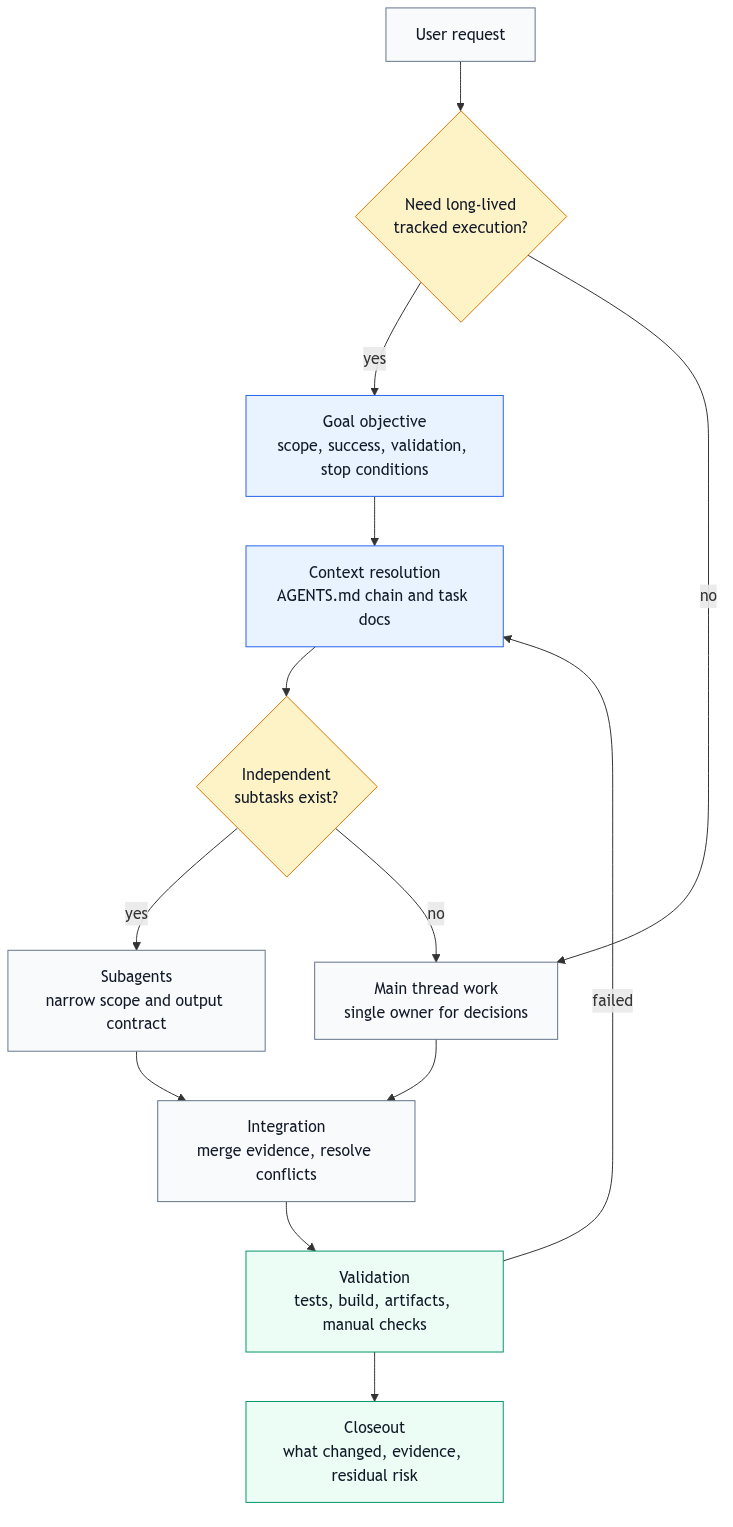
\includegraphics[height=0.76\textheight]{goal-subagent-flow.png}
  \caption{Goal 生命周期与 subagent 分工的组合流程}
\end{figure}

如果任何一步没有足够信息，就不要进入下一步。例如没有 validation，就不能可靠 closeout；没有 write scope，就不能安全 dispatch；没有 stop conditions，就容易在权限或证据不足时硬做。

\subsection{组合时的常见错误}

\begin{itemize}
  \item \keypoint{把 Goal 当标题}：只写“优化系统”没有 scope、validation、stop conditions。
  \item \keypoint{把 subagent 当廉价并行}：多个 agent 改同一批文件，最后产生冲突。
  \item \keypoint{让 subagent 接管生命周期}：subagent 创建 goal、创建 worktree、自己 merge，这是边界错误。
  \item \keypoint{没有 AGENTS.md chain}：subagent 不知道局部规则，容易破坏项目约定。
  \item \keypoint{没有整合证据}：多个 agent 都说完成，但主线程没有重新跑测试。
\end{itemize}

\subsection{什么时候不要用 Goal 或 subagent}

不要把所有任务都升级成 Goal 或 subagent：

\begin{itemize}
  \item 一行命令能回答的问题，用普通会话；
  \item 单文件小改且验证简单，用普通会话；
  \item 只是询问建议，用 report-only 或 plan-only；
  \item 边界不清楚，先 grill 或问问题；
  \item 没有独立子任务，不要为了形式创建 subagents。
\end{itemize}

\section{项目配置：怎么写 \file{AGENTS.md}}

\file{AGENTS.md} 是 Codex 的项目说明书。Codex 在开始工作前读取 instructions；全局、项目根、子目录 instructions 会形成一条 instruction chain，离当前目录更近的文件优先级更高。

\subsection{发现顺序}

可以按三层理解：

\begin{enumerate}
  \item \keypoint{全局层}：默认在 \file{\textasciitilde/.codex/} 下读取 \file{AGENTS.override.md} 或 \file{AGENTS.md}。
  \item \keypoint{项目层}：从 Git root 或项目 root 往当前目录走，每层最多读一个 instructions 文件。
  \item \keypoint{就近覆盖}：越靠近当前工作目录的 \file{AGENTS.md} 越晚进入上下文，因此能覆盖更上层规则。
\end{enumerate}

如果项目很大，不要把所有规则都塞到根目录一个超长文件里。根 \file{AGENTS.md} 放共识，子目录放局部规则。

\subsection{项目根 \file{AGENTS.md} 模板}

一个实用的项目根文件可以这样写：

\begin{lstlisting}
# AGENTS.md

## Repository Expectations

- Start by reading README.md and the nearest AGENTS.md.
- Preserve unrelated dirty worktree changes.
- Prefer rg / rg --files for search.
- Use apply_patch for manual edits.

## Build And Test

- Python: python3 -m pytest
- Frontend: npm run build
- Quality: make lint

## Verification

Before claiming completion, report:
- files changed
- commands run
- tests passed or why they could not run
- remaining risks

## Review Policy

For review requests, list findings first with file/line references.
Prioritize correctness, security, regressions, and missing tests.

## Documentation

- Domain terms live in CONTEXT.md.
- Durable decisions live in docs/adr/.
- Task process notes live under doc/.
\end{lstlisting}

\subsection{子目录 \file{AGENTS.md}}

只有当某个目录真的有不同规则时才加：

\begin{itemize}
  \item \file{frontend/AGENTS.md}：规定 UI 构建、截图验证、设计系统、浏览器测试。
  \item \file{backend/AGENTS.md}：规定 API 兼容、数据库迁移、服务端测试。
  \item \file{paper/AGENTS.md}：规定 LaTeX 编译、证据边界、引用审计。
  \item \file{experiments/AGENTS.md}：规定 GPU、数据路径、离线模式、日志和结果保存。
\end{itemize}

不要写空洞规则，例如“写高质量代码”。要写可执行规则，例如“改 API 后必须跑 \cmd{python3 -m pytest tests/test\_api.py}”。

\subsection{验证 \file{AGENTS.md} 是否生效}

最简单的验证方式：

\begin{lstlisting}
在 Codex Desktop 当前线程里询问：
"Summarize the current instructions and list active AGENTS.md files."

切到目标子目录后再询问：
"Show which instruction files apply to this path before editing."
\end{lstlisting}

如果 Codex 行为看起来像没读规则，先检查：

\begin{itemize}
  \item 是否在正确项目目录启动；
  \item 文件是否为空；
  \item 是否有更高优先级的 \file{AGENTS.override.md}；
  \item instruction 文件是否太长被截断；
  \item 是否需要重启当前 Codex session。
\end{itemize}

\section{日常任务请求与验证}

普通 Codex 请求也应该有结构。越清楚的请求，越少返工。

\subsection{一个好请求的结构}

最稳的请求包含四件事：

\begin{itemize}
  \item \keypoint{目标}：要产出什么，例如“修复这个测试”、“写一份 LaTeX 指南”、“把这个 PR 合进去”。
  \item \keypoint{范围}：在哪个仓库、哪个模块、哪些文件内工作。
  \item \keypoint{约束}：不能改什么、必须保留什么、输出语言、字符数、公开 API、字段名、路径边界。
  \item \keypoint{验证}：希望跑哪些测试、构建命令，或接受什么检查作为完成证据。
\end{itemize}

示例：

\begin{lstlisting}
在 /home/hujie/paper/tools/codex-usage-guide 里重写 LaTeX 指南。
中文优先，保留英文技能名。Goal 和 subagent 内容放前面，
后面再介绍工程和学术 skills。最后重新 make pdf 并检查中文抽取。
\end{lstlisting}

\subsection{看 Codex 是否靠谱}

不要只看它是否说“完成”。要看三个证据：

\begin{itemize}
  \item 它是否读了正确入口：\file{AGENTS.md}、\file{README.md}、\file{pyproject.toml}、\file{package.json}、相关 \file{SKILL.md}。
  \item 它是否只修改任务相关文件，并保留 unrelated dirty worktree。
  \item 它是否运行了合适验证，并说明失败是代码问题、依赖问题、权限问题还是外部服务问题。
\end{itemize}

\subsection{权限请求怎么判断}

Codex 请求批准时，先看命令的影响面：

\begin{itemize}
  \item 是否访问网络或下载依赖；
  \item 是否写工作区外目录；
  \item 是否删除、重置或覆盖文件；
  \item 是否启动长期服务或实验；
  \item 是否可以用更窄的命令完成。
\end{itemize}

持久授权要窄。例如授权 \cmd{npm run dev} 通常比授权整个 \cmd{python3} 更安全。

\section{工程场景：Matt Pocock skills 流程}

从这里开始是场景化 skills 使用。工程场景主要使用 Matt Pocock 风格 skills。它们的路由入口是 \skill{ask-matt}，核心思想是：先把 idea 问清楚，再把工作拆成可交付的问题，最后实现和审查。

\subsection{\skill{grill-me} 与 \skill{grill-with-docs}}

\skill{grill-me} 是无状态拷问：适合没有代码仓库、只是要打磨计划或设计的时候。它不会写 \file{CONTEXT.md}，也不会沉淀 ADR。

\skill{grill-with-docs} 是有仓库上下文的拷问：适合一个设计已经落在代码库里，需要一边追问、一边把术语写入 \file{CONTEXT.md}，必要时写 \file{docs/adr/}。

简单判断：

\begin{itemize}
  \item 没有代码库，只想磨方案：用 \skill{grill-me}。
  \item 有代码库，术语、接口、架构选择会影响后续维护：用 \skill{grill-with-docs}。
  \item 不知道该走哪条：先用 \skill{ask-matt}。
\end{itemize}

\subsection{工程主流程}

工程主流程可以记成这一条线：

\begin{lstlisting}
grill-with-docs 或 grill-me
  -> handoff / prototype
  -> to-prd
  -> to-issues
  -> implement
  -> review / finishing-a-development-branch
\end{lstlisting}

每一步的职责不同：

\begin{itemize}
  \item \skill{grill-with-docs}：压实问题、术语和架构边界。
  \item \skill{handoff}：把长会话压成可跨会话继续的 Markdown。
  \item \skill{prototype}：用一次性代码验证不确定的状态模型、交互或业务逻辑。
  \item \skill{to-prd}：把稳定想法写成产品或工程需求。
  \item \skill{to-issues}：把 PRD 拆成可独立领取的 issue。
  \item \skill{implement}：按单个 issue 实现，不把所有上下文都塞进一个超长会话。
  \item \skill{review}：以问题、风险、缺失测试为主做审查。
\end{itemize}

\subsection{工程纪律}

\begin{itemize}
  \item \keypoint{先问清楚，不急着写代码}：架构、接口、术语不清楚时，先 grill。
  \item \keypoint{把大任务拆成 issues}：多会话、多模块任务不要靠一个巨大上下文硬撑。
  \item \keypoint{每个 issue fresh context}：实现阶段以 issue 和 PRD 为输入，减少历史会话污染。
  \item \keypoint{review 先找风险}：review 的第一输出应该是 bug、回归、缺失测试和行为风险。
  \item \keypoint{文档只记录稳定事实}：\file{CONTEXT.md} 是术语表，不是 todo list；ADR 只记录难回退、有取舍、未来会追问的决定。
\end{itemize}

\subsection{工程 skills 的具体使用例子}

例子一：你只有一个模糊想法，还没有代码仓库。

\begin{lstlisting}
[$grill-me]
我想做一个 Codex 使用指南，但现在不知道目标读者、章节结构、
是否需要 PDF 和 GitHub Pages。请一次只问一个问题，先帮我把边界问清楚。
\end{lstlisting}

这类请求适合 \skill{grill-me}，因为它的目标是压实想法，不需要维护项目文档。

例子二：你已经有仓库，需要让设计沉淀到文档里。

\begin{lstlisting}
[$grill-with-docs]
仓库在 /home/hujie/paper/tools/codex-usage-guide。
我要把指南改成 GitHub 可发布的中文文档站。
请先读 README.md、CONTEXT.md、AGENTS.md，再追问设计边界；
稳定术语写入 CONTEXT.md，重要结构决策写入 docs/adr/。
\end{lstlisting}

这类请求适合 \skill{grill-with-docs}，因为后续维护者需要知道术语、边界和架构决定从哪里来。

例子三：设计已经稳定，需要拆成实现单元。

\begin{lstlisting}
[$to-prd]
基于当前 CONTEXT.md 和 ADR，把 Codex 使用指南网页化写成 PRD。
要求覆盖：侧边栏导航、卡片跳转、Goal 示例、research-pipeline 示例、
GitHub Pages 发布边界、PDF 构建验证。

[$to-issues]
把上面的 PRD 拆成 3-5 个可独立实现的 issues。
每个 issue 要有范围、验收标准、验证命令和不允许修改的边界。
\end{lstlisting}

拆成 issues 后，再用 \skill{implement} 逐个实现。这样比把“网页、PDF、仓库、发布、审查”全部塞进一个会话更稳。

\section{学术场景：research skills}

学术自动化不要套用工程 issue 流程。论文工作更强调研究问题、新颖性、证据边界、实验可信度和投稿风险。本机已经有两层路由：\skill{academic-research-suite} 和 \skill{ask-research}。

\subsection{\skill{academic-research-suite}}

\skill{academic-research-suite} 是 Codex-native ARS 总入口。它不会默认加载整套材料，而是根据任务选择一个 workflow：

\begin{itemize}
  \item \skill{deep-research}：文献综述、系统综述、meta-analysis、研究问题收敛、事实核查。
  \item \skill{academic-paper}：论文大纲、摘要、正文、修订、引用格式、AI disclosure、格式转换。
  \item \skill{academic-paper-reviewer}：模拟审稿、editorial decision、re-review。
  \item \skill{academic-pipeline}：从研究到论文的端到端流程和 integrity gate。
  \item \skill{experiment-agent}：实验计划、代码实验执行计划、人类研究 protocol、统计解释、可复现性验证。
\end{itemize}

\subsection{\skill{ask-research}}

\skill{ask-research} 是本机 AI/ML 论文研究路由器。它不重写下游流程，而是帮你选正确 skill。

常见路径：

\begin{itemize}
  \item 早期 idea 或投稿前强审：\skill{research-grill-me}。
  \item 模糊方向到方法和实验：\skill{research-refine-pipeline}。
  \item 实验计划：\skill{experiment-plan}。
  \item 启动少量实验：\skill{run-experiment}。
  \item 大批量实验：\skill{experiment-queue}。
  \item 监控实验：\skill{monitor-experiment}。
  \item 结果到 claim：\skill{result-to-claim}。
  \item claim 证据检查：\skill{paper-claim-audit}、\skill{paper-evidence-boundary-sync}。
  \item 写作和修订：\skill{paper-write}、\skill{paper-writing}、\skill{academic-prose-degenericizer}。
  \item 投稿前引用和编译：\skill{citation-audit}、\skill{paper-compile}。
  \item rebuttal：\skill{rebuttal}。
\end{itemize}

\subsection{\skill{research-grill-me}}

\skill{research-grill-me} 是中文主导的 AI/ML 论文强门槛流程。它像 \skill{grill-with-docs} 一样一次只问一个问题，同时维护研究文档。

它覆盖这些 gate：

\begin{itemize}
  \item Idea Gate：问题是否值得做；
  \item Literature / Novelty Gate：closest work 是否压塌新颖性；
  \item Method Gate：方法机制是否必要；
  \item Experiment Gate：baseline、ablation、metric、seed 和算力是否足够；
  \item Result / Claim Gate：结果能否支撑 claim；
  \item Paper Gate：故事线、图表、limitations 和 venue framing；
  \item Submission Gate：投稿前 red-team；
  \item Rebuttal / Migration Gate：审稿回复和转投策略。
\end{itemize}

它会维护 \file{docs/research\_dossier.md}、\file{CONTEXT.md} 和必要 ADR。结论可以是 \skill{STOP}、\skill{PIVOT}、\skill{LITERATURE FIRST}、\skill{EXPERIMENT FIRST} 或 \skill{READY}。这比“帮我润色论文”更早、更严格。

\subsection{\skill{research-pipeline}：从找 idea 到投稿}

\skill{research-pipeline} 是更完整的研究生命周期入口。它把 idea discovery、实现、实验部署、自动 review loop 和可选论文写作串成一个端到端流程。适合用户明确说“全流程”“从找 idea 到投稿”“end-to-end research”，或者希望在一个研究方向上持续推进到 submission-ready paper。

它的核心链路是：

\begin{lstlisting}
idea-discovery
  -> implement
  -> run-experiment / experiment-queue
  -> auto-review-loop
  -> NARRATIVE_REPORT.md
  -> paper-writing (optional)
\end{lstlisting}

常用参数要先想清楚：

\begin{itemize}
  \item \keypoint{AUTO\_PROCEED}：是否在 idea 阶段自动选择排名第一的 idea。初次使用建议设为 \skill{false}。
  \item \keypoint{HUMAN\_CHECKPOINT}：auto-review 每轮后是否暂停给人类看分数和修改意见。
  \item \keypoint{REVIEWER\_DIFFICULTY}：review 难度，\skill{medium} 适合常规迭代，\skill{nightmare} 适合投稿前强审。
  \item \keypoint{AUTO\_WRITE}：是否自动进入论文写作。默认 \skill{false} 更安全，因为论文故事线和 venue framing 常需要人工确认。
  \item \keypoint{VENUE}：当 \skill{AUTO\_WRITE=true} 时必须明确，例如 \skill{ICLR}、\skill{NeurIPS}、\skill{CVPR}。
\end{itemize}

例子一：安全的半自动研究流水线。

\begin{lstlisting}
[$research-pipeline]
方向：长上下文 LLM 推理中的 KV cache pruning。
AUTO_PROCEED: false
HUMAN_CHECKPOINT: true
REVIEWER_DIFFICULTY: hard
AUTO_WRITE: false

请先生成 idea-stage/IDEA_REPORT.md，列出 top ideas、closest work、
pilot 信号和推荐理由。不要在我确认 idea 前进入 full experiment。
\end{lstlisting}

这个写法适合零到一探索：先把 idea 和 novelty 摆出来，人确认后再花 GPU。

例子二：夜间自动实验和 review。

\begin{lstlisting}
[$research-pipeline]
方向：MoE 模型专家路由压缩。
AUTO_PROCEED: true
HUMAN_CHECKPOINT: false
REVIEWER_DIFFICULTY: medium
AUTO_WRITE: false

如果 Stage 1 排名第一的 idea 同时满足 novelty confirmed 和 pilot positive，
自动进入实现、实验部署和 auto-review-loop。记录 GPU-hours，
最终生成 NARRATIVE_REPORT.md 和 review-stage/AUTO_REVIEW.md。
\end{lstlisting}

这个写法适合“晚上启动，早上看结果”。但如果算力昂贵或题目敏感，应把 \skill{AUTO\_PROCEED} 改成 \skill{false}。

例子三：投稿前强审，但不自动写论文。

\begin{lstlisting}
[$research-pipeline]
方向：已有 repo 中的 pruning 方法是否能投 NeurIPS。
AUTO_PROCEED: false
HUMAN_CHECKPOINT: true
REVIEWER_DIFFICULTY: nightmare
AUTO_WRITE: false

请优先检查 novelty、baseline、ablation、metric、seed、claim-evidence。
如果 auto-review-loop 到第 4 轮仍不到 6/10，停止并列出 blocker。
\end{lstlisting}

\skill{research-pipeline} 的关键产物不是“模型说可以投”，而是 \file{IDEA\_REPORT.md}、实验结果、\file{AUTO\_REVIEW.md}、\file{NARRATIVE\_REPORT.md} 和剩余 blocker。没有这些证据，不要把结论写成 submission-ready。

\subsection{学术安全边界}

\begin{itemize}
  \item 不把未发表 manuscript、reviewer comments 或私有语料上传到外部模型，除非用户明确同意。
  \item 没有 live literature search 或明确 closest-work packet 时，新颖性不能标成 strong。
  \item claim 必须绑定具体 evidence；没有证据的宏大叙述要降级或删除。
  \item 实验结果、日志、表格和论文文本要区分：结果存在，不等于 claim 已经安全。
\end{itemize}

\section{模式选择速查}

\begin{itemize}
  \item \keypoint{简单问答或单文件小改}：普通 Codex 会话即可。
  \item \keypoint{工程 idea 不清楚}：无代码库用 \skill{grill-me}；有代码库用 \skill{grill-with-docs}。
  \item \keypoint{工程大任务}：\skill{ask-matt} 路由到 grill、PRD、issues、implement、review。
  \item \keypoint{AI/ML 论文研究}：\skill{ask-research} 或 \skill{academic-research-suite}。
  \item \keypoint{论文强门槛拷问}：\skill{research-grill-me}。
  \item \keypoint{从找 idea 到实验、review、写作 handoff}：\skill{research-pipeline}。
  \item \keypoint{多个独立实现任务}：\skill{subagent-driven-development}。
  \item \keypoint{多个独立故障调查}：\skill{dispatching-parallel-agents}。
  \item \keypoint{长流程、强审计、需要目标闭环}：优先使用通用 Goal 模式或可复现插件；本机 \skill{goal-entry} 只是自开发实验，效果一般，具体见最后一节。
\end{itemize}

\section{官方资料与维护方法}

本指南当前参考了这些来源：

\begin{itemize}
  \item OpenAI Codex app 官方页面：\url{https://developers.openai.com/codex/app}
  \item OpenAI Codex manual：\url{https://developers.openai.com/codex/codex-manual.md}
  \item 本机 skills：\file{/home/hujie/.codex/skills/ask-matt/SKILL.md}
  \item 本机 skills：\file{/home/hujie/.codex/skills/academic-research-suite/SKILL.md}
  \item 本机 skills：\file{/home/hujie/.codex/skills/research-pipeline/SKILL.md}
  \item 本机 skills：\file{/home/hujie/.codex/skills/subagent-driven-development/SKILL.md}
  \item Compound Engineering plugin：\url{https://github.com/EveryInc/compound-engineering-plugin}
  \item 自开发 \skill{goal-entry} 实验仓库：\url{https://github.com/WhoJay0609/codex-goal-entry}
\end{itemize}

\subsection{本机自写或本地维护 skills 备注}

本文提到的 skills 不是同一种来源。Codex app、worktree、automation、in-app browser、review 等属于产品或官方能力；Compound Engineering 属于第三方插件；而 \skill{ask-research}、\skill{research-grill-me}、部分 Matt Pocock 风格 workflow、本机 \skill{goal-entry} 和若干 \file{goal-*} skills 属于本机安装、本地维护或自写扩展。其中 \skill{goal-entry} 是自己开发的实验，实际效果一般，不应被理解成 OpenAI 官方内置功能或推荐默认路径。

使用这些本机 skills 时，优先级应该是：

\begin{enumerate}
  \item 先读当前机器上的 \file{SKILL.md}，不要只凭这份指南或旧记忆。
  \item 看它是否要求读取额外 reference、template、script 或 assets。
  \item 如果 skill 是本机自写或本地维护，向团队或读者说明“这是本仓库/本机器工作流的一部分”，避免把它当成通用 Codex 标准。
  \item 如果要发布到 GitHub，把本机路径、私有约定和不可复现命令标成“local adaptation”或放入单独附录。
\end{enumerate}

本指南最后一节只保留本机 \skill{goal-entry} 的简要实现说明；前面的 Goal、subagent 和插件章节保持通用，方便没有安装这些本机 skills 的读者也能学习。

本指南会过期，尤其是 skills 名称、Goal 使用方法、ARS workflow 和本地 MCP 工具。维护时先查 live 文件，而不是凭记忆改：

\begin{itemize}
  \item 工程流：读 \file{/home/hujie/.codex/skills/ask-matt/SKILL.md} 和 Matt 相关 skills。
  \item 学术流：读 \file{academic-research-suite/SKILL.md}、\file{ask-research/SKILL.md}、\file{research-pipeline/SKILL.md}。
  \item 研究拷问：读 \file{research-grill-me/SKILL.md}。
  \item subagent 流：读 \file{subagent-driven-development/SKILL.md}。
  \item 并行 agent：读 \file{dispatching-parallel-agents/SKILL.md}。
  \item Goal 入口实现：见最后一节，再读对应本机 skill 文件。
\end{itemize}

重新编译：

\begin{lstlisting}
make pdf
\end{lstlisting}

\section{本机 \skill{goal-entry} 对应实现}

本节是全文最后一节，只把前面的通用 Goal/Subagent 模型映射到本机实现。当前本机入口是 \skill{goal-entry}，但它是自己开发的 local adaptation，效果一般，不建议作为默认学习路径。它是 router-only public entry，不把所有规则写在自己文件里，而是先用 resolver 分类，再路由到子 skill。公开版本仓库见：\url{https://github.com/WhoJay0609/codex-goal-entry}。

\subsection{本机实现备注}

\skill{goal-entry} 和相关 \skill{goal-*} skills 是本机维护的目标编排层，不是每个 Codex 安装环境都会自带的官方标准接口。阅读本节时应把它看成“一个效果一般的本地实验案例”：通用原则是 Goal objective、readiness、context、dispatch、validation 和 closeout；具体脚本名、路径和路由规则以本机 \file{SKILL.md} 为准。

\subsection{\skill{goal-entry} 如何对应前文概念}

前文通用概念和本机实现的对应关系如下：

\begin{itemize}
  \item \keypoint{请求分类}：由 \file{resolve\_goal\_entry.py} 判断 request mode、tier、dispatch level、readiness 和 goal action。
  \item \keypoint{准备检查}：由 \skill{goal-preflight} 检查 objective 长度、repo/path、AGENTS/doc context 和 readiness。
  \item \keypoint{Goal objective}：由 \skill{goal-objective} 生成紧凑 objective。本机硬规则是不超过 4,000 字符。
  \item \keypoint{项目 instructions}：由 \skill{goal-context} 解析 \file{AGENTS.md} 层级和路径索引。
  \item \keypoint{团队和 subagent 边界}：由 \skill{goal-team} 和 \skill{goal-dispatch} 负责团队选择、dispatch contract、write scope 和输出合同。
  \item \keypoint{运行 artifact}：由 \skill{goal-backend} 维护 artifact-producing run。
  \item \keypoint{验证和收尾}：由 \skill{goal-trace} 与 \skill{goal-close} 处理验证证据和 closeout。
\end{itemize}

\subsection{\skill{goal-entry} 的路线}

\skill{goal-entry} 的关键流程：

\begin{lstlisting}
goal-entry
  -> resolve_goal_entry.py
  -> goal-preflight
  -> goal-objective
  -> goal-context
  -> goal-team / goal-dispatch
  -> goal-backend
  -> goal-trace / goal-close
\end{lstlisting}

\subsection{\skill{goal-entry} 的硬规则}

\begin{itemize}
  \item 不创建嵌套 Codex goals。
  \item readiness 不明确时不调用 \skill{create\_goal}。
  \item objective 不超过 4,000 字符。
  \item subagent 不允许调用 \skill{get\_goal}、\skill{create\_goal}、\skill{update\_goal}。
  \item subagent 不允许被分配 \skill{goal-*} 或 legacy harness protocol skills。
  \item 不绕过 \file{resolve\_goal\_entry.py} 手写 mode logic。
  \item 对 \skill{execute\_goal} 或 \skill{active\_goal\_bind} 不绕过 \skill{goal-preflight}。
\end{itemize}

\subsection{什么时候直接点名 \skill{goal-entry}}

当请求需要先分类再决定是否创建 goal、绑定 active goal、规划、dispatch、初始化 backend artifact 或 closeout 时，可以直接点名：

\begin{lstlisting}
[$goal-entry](https://github.com/WhoJay0609/codex-goal-entry)
请先判断这是 plan-only 还是 execute_goal。
如果需要执行，先给出 compact objective 和 stop conditions。
\end{lstlisting}

如果只是简单问答，不要点名 \skill{goal-entry}。如果只是想要一份计划，也不要让它创建 goal；让它走 \skill{goal-plan} 或 plan-only handoff。

\subsection{\skill{goal-entry} 的具体使用例子}

例子一：先判断是否需要创建 Goal。

\begin{lstlisting}
[$goal-entry]
请先判断这是 plan-only 还是 execute_goal。
任务：把 codex-usage-guide 的网页改成中文侧边栏文档站，
并在完成后重新构建、推送、检查 GitHub Pages。

如果需要执行，请给出 compact objective、validation 和 stop conditions。
\end{lstlisting}

这类请求不应该直接开干。正确流程是先由 resolver 判断 \skill{request\_mode}、\skill{goal\_entry\_tier}、\skill{goal\_action}，再决定是否进入 preflight 和 goal creation。

例子二：明确只是计划。

\begin{lstlisting}
[$goal-entry]
只规划，不执行。请给出把 goal-entry 拆成公开仓库的计划：
范围、文件清单、隐私检查、验证命令、GitHub 发布步骤。
\end{lstlisting}

这个请求应当走 \skill{plan\_only} 或 handoff，不应该调用 \skill{create\_goal}。

例子三：带验收的执行目标。

\begin{lstlisting}
[$goal-entry]
执行：创建 goal-entry 的公开仓库，推送到 GitHub；
然后更新 codex-usage-guide，在介绍 goal-entry 时链接新仓库。

验收：
- 新仓库公开可访问；
- resolver quick_validate 通过；
- codex-usage-guide 的 PDF 和 GitHub Pages 都更新；
- 最终报告链接、提交 hash 和验证结果。
\end{lstlisting}

这个请求适合 \skill{execute\_goal}：它有跨仓库修改、公开发布、验证和 closeout，应该有明确 objective 和停止条件。

\subsection{维护时读取的本机文件}

\begin{itemize}
  \item \file{/home/hujie/.codex/skills/goal-entry/SKILL.md}
  \item \file{/home/hujie/.codex/skills/goal-objective/SKILL.md}
  \item \file{/home/hujie/.codex/skills/goal-dispatch/SKILL.md}
  \item \file{/home/hujie/.codex/skills/goal-team/SKILL.md}
  \item \file{/home/hujie/.codex/skills/goal-preflight/SKILL.md}
\end{itemize}

\end{document}
